\subsection{Interfaces}
\index{Interfaces}

An interfaces is a defect between materials with different properties, or between a material and the lack of it (a free interface).

\subsubsection{Parameters}

Interface defects are not user-specified. They are build by default between materials with different names. For a free interface, the special material \param{Gas} can be used. 

Because an interface involves two materials, the interface parameters are defined in folders that are created by appending the name of both materials separated with an underline ``\verb+_+'', in alphabetical order. This way, an interface between Iron and Gas would be parametrized under the {\tt Gas\verb+_+Iron} name.

Each material folder contains the parameters for each element that can interact with the interface. The parameters allowed for these elements are listed below. The parameter \param{left} is important, because it defines what is called ``left'' in the parameters using it. This way, if \param{left} is set to ``Iron'', any param finishing in ``left'' will refer to ``Iron'', and ``right'' will refer about the other material in the interface, independently on the name of the folder. 

For instance, in {\tt Iron\verb+_+Gas} if \param{left} is Iron, then any reference to ``right'' will refer to Gas. In {\tt Copper\verb+_+Iron}, if \param{left} is also Iron, ``right'' will mean Copper. As you can see, this is independent on whether the folder name (ordering the names alphabetically) starts or finishes with Iron.

\begin{description}
\item[\param{barrier.left}] The (extra) energetic barrier to be overcome to react with the interface.
\item[\param{barrier.right}] See barrier.left.
\item[\param{desorption.high}] See desorption.threshold.
\item[\param{desorption.low}] See desorption.threshold
\item[\param{desorption.threshold}] For surface concentrations lower than this value, the parameter \param{desorption.low} will be used. Otherwise \param{desorption.high} will be applied. Desorption is the probability for a particle to be annihilated at the surface.
\item[\param{formation}] The formation energy of the impurity when trapped at the interface. The particle will be emitted to either side depending on the difference of energies between this formation energy and the formation energy in the materials at either side.
\item[\param{left}] Definition of which material is considered left, independently on the name of the folder for the interface.
\item[\param{migration}] Migration energy and prefactor for the inpurity on the interface.
\item[\param{recombination.lenght.left}] For self-interstitials and self-vacancies, defines the sink efficiency at the interface.
\item[\param{recombination.lenght.right}] See recombination.lenght.left.
\end{description}

A graphical description of the meaning of these parameters can be seen in Fig.~\ref{fig:interface}

\begin{figure}
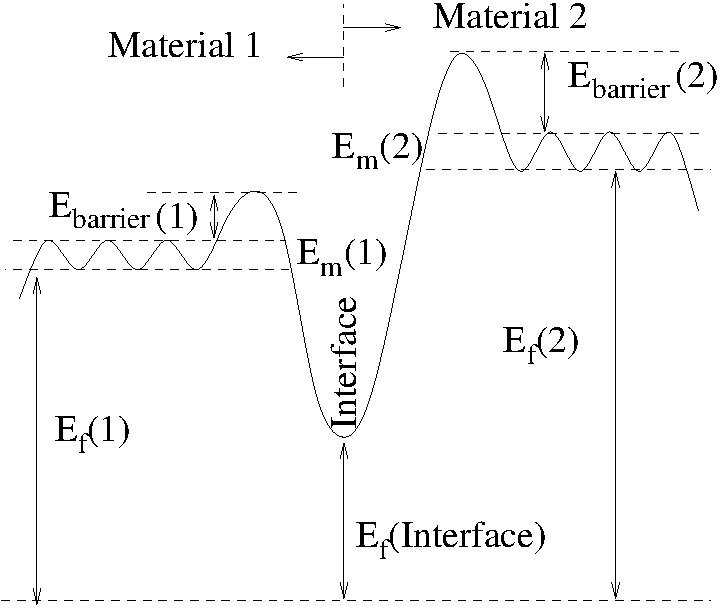
\includegraphics{images/interface}
\caption{Energies involved at the interface reactions.}
\label{fig:interface}
\end{figure}


\subsubsection{Interactions}

The interactions with interfaces are defined in the {\param Models} file for each side of such interface. The syntax for them is
\begin{lstlisting}
Defect+MaterialFullName true/false
\end{lstlisting}
the full name for the material is to be used. This way the syntax checker can distinguish between the interaction with an interface (for instance, {\tt I+Iron}, or with an impurity of the same material {\tt I+Fe}.


As an example, in the case of a {\tt Copper\verb+_+Iron} interface, at the {\tt Iron} side, the interaction with the material  is defined at {\tt Iron/Models/interactions} as
\begin{lstlisting}
Defect+Copper true
\end{lstlisting}
being {\tt Defect} the defect being considered (I, V, ICluster, etc...). Similarly, at the Copper side we will see
\begin{lstlisting}
MP+Iron true
\end{lstlisting}

\subsubsection{Conclusions}
Interfaces are 2D planar objects isolating one material from a different one. Mobile particles and clusters are allowed to interact with them. For mobile particles, they can be annihilated, or trapped and re-emitted to either side. For clusters they can only be annihilated (desorption). 

